\subsection{\spatialAcronym: direct solution approach}\label{sec:direct} 
\KTC{HERE}
\KTC{Does the time grid definted in this section have any relationship to the
time grid used for time discretization? Haven't gotten past HERE below, but
wanted to check (maybe it's made clear later).}
\EP{This time grid becomes the time discretization over each window. At this point in the paper, 
there is no notion of a time grid for \methodAcronym}

Direct approaches solve the optimization problem~\eqref{eq:tclsrm} by
``transcribing" the infinite dimensional optimization problem into a finite
dimensional one by discretizing the state and objective functional in time.
The minimization problem is then reformulated as a (non)linear programming, or
optimization, problem. A variety of direct solution approaches exist, 
including collocation approaches, spectral  methods, and genetic algorithms.  

In the present context, the most straightforward direct solution approach consists of the 
following steps: (1) numerically discretize the FOM ODE (and hence the \textit{integrand} of~\eqref{eq:obj_gen_slab}) and 
(2) select a numerical quadrature rule to evaluate the \textit{integral} in~\eqref{eq:obj_gen_slab}.
To this end, we start by defining a discrete time grid 
over each window by introducing
$\nstepsArg{n}+1$ strictly increasing time instances described by
$\{\timeWindowArg{n}{i}\}_{i=0}^{\nstepsArg{n}}$ with
%\KTC{use cdots, not
%hdots or ldots. Don't use $\defeq$ for the first and last times; these are
%just equalities, i.e., you happen to set them equal to those values, but they
%aren't identically the same:}
\begin{align}
&\timeWindowArg{n}{0} \le \cdots \le \timeWindowArg{n}{\nstepsArg{n}} , \label{eq:timegrid1} \;
\timeWindowArg{n}{0} = \timeStartArg{n},\;
\timeWindowArg{n}{\nstepsArg{n}} = \timeEndArg{n} . 
%\timeWindowArg{n}{0} = \timeStartArg{n}, \timeWindowArg{n}{\nstepsArg{n}} =
%\timeEndArg{n}
\end{align}
Figure~\ref{fig:slab_fig2} depicts this discretization.
We now outline the direct solution approach for linear-multistep schemes; we note that the formulation for
other time-stepping methods (e.g., Runge--Kutta) follows closely. 
\begin{figure} 
\begin{centering} 
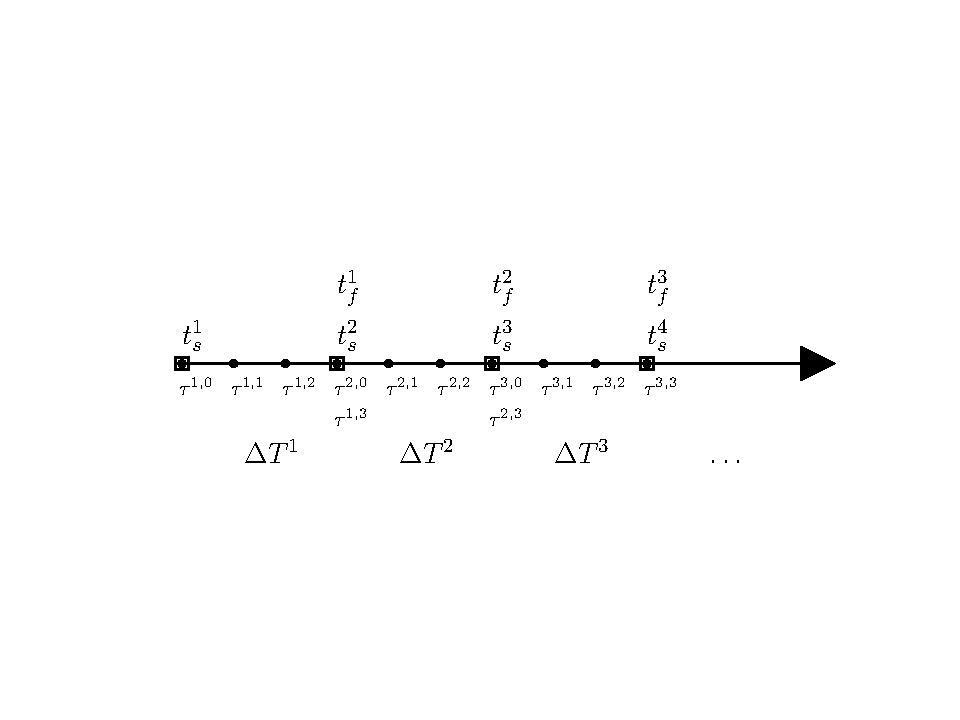
\includegraphics[trim={0.0cm 4.5cm 0cm 3cm},clip,width=1.0\textwidth]{figs/time_grid_timesteps.pdf} 
	\caption{Depiction of the $\nstepsArg{n}+1$ time instances over each window. In the figure, $\nstepsArg{n} = 2$ for all $n$.} 
\label{fig:slab_fig2} 
\end{centering} 
\end{figure}
%We now outline several commonly employed temporal discretization 
%schemes, specifically linear multistep and collocation (Runge--Kutta) methods, that leverage this time-grid to discretize the FOM ODE and 
%objective functional.  

%\subsubsection{Temporal Discretization of the FOM ODE}
%To develop the direct solution approach, we first outline several 
%commonly employed methods used to discretize the FOM ODE, and then 
%subsequently demonstrate how these techniques can be used to discretize 
%and solve Eq.~\ref{eq:obj_gen_slab}. To develop the direct solution approach, 
%we start by dividing each time slab $[\timeStartArg{n},\timeEndArg{n}]$ into
%$\nstepsArg{n}$ strictly increasing time-step instances described by,
%$\{\timeWindowArg{n}{i}\}_{i=0}^{\nstepsArg{n}}$, with  \begin{align*}
%&\timeWindowArg{n}{0} \le \ldots \le \timeWindowArg{n}{\nstepsArg{n}} , \\
%&\timeWindowArg{n}{0} \defeq \timeStartArg{n}, \\
%&\timeWindowArg{n}{\nstepsArg{n}} \defeq \timeEndArg{n}. 
%%\timeWindowArg{n}{0} = \timeStartArg{n}, \timeWindowArg{n}{\nstepsArg{n}} =
%%\timeEndArg{n}
%\end{align*}
\subsubsection{Linear multistep schemes}
\EP{This section has the double superscript. We could make one of these a subscript, but then need to change the algorithms a bit as 
I use subscripts to denote iterations. Either is fine}
Linear multistep schemes approximate the solution at time instance $\timeWindowArg{n}{i}$ using the previous $k$ time instances.  
%Discretizing the FOM ODE~\eqref{eq:FOM} with a linear $k$-step scheme at the $i$th time-instance over the $n$th time slab yields,
%\begin{equation}\label{eq:kstep}
%\sum_{j=0}^{\lmsWidthArg{n}{i}} \alpha_j \stateFOMDiscreteArg{n,i-j} = \Delta t^{n,i} \sum_{j=0}^{\lmsWidthArg{n}{i}} \beta_j \velocity(\stateFOMDiscreteArg{n,i-j}),
%\end{equation}
Employing a linear multistep method for temporal discretization of the FOM ODE yields the FOM O$\Delta$E over the $n$th window,
\begin{align*}
&\residLMSArg{n,i} (\stateFOMDiscreteArg{n,i},\ldots,\stateFOMDiscreteArg{n,i-\lmsWidthArg{n}{i}}) = \bz, \qquad i=1,\ldots,\nstepsArg{n}, \\
&\stateFOMDiscreteArg{n,0} = \begin{cases}
\stateFOMDiscreteArg{n-1,\nstepsArg{n-1}} & n = 2,\ldots,\nslabs, \\
\stateFOMIC & n=1, \end{cases}
\end{align*}
where $\stateFOMDiscreteArg{n,i} \approx \stateFOMArg{}{\timeWindowArg{n}{i}} \in \RR{\fomdim}$ is the discrete approximation to the FOM state at the $i$th time instance over the $n$th window and $\residLMSArg{n,i}$ is the discrete linear multistep residual over the $i$th time instance of the $n$th window and is defined as
\begin{align*}
\residArg{n,i} &: (\stateyDiscreteArgnt{i},\ldots,\stateyDiscreteArgnt{i-\lmsWidthArg{n}{i}}) \mapsto  \frac{1}{\Delta t^{n,i}} \sum_{j=0}^{\lmsWidthArg{n}{i}} \alpha^{n,i}_j \stateyDiscreteArgnt{i-j} -  \sum_{j=0}^{\lmsWidthArg{n}{i}} \beta^{n,i}_j \velocity(\stateyDiscreteArgnt{i-j},\timeWindowArg{n}{i-j}) \\
               &: \RR{\fomdim} \otimes \RR{\lmsWidthArg{n}{i}+1} \rightarrow \RR{\fomdim}. 
\end{align*} 
Additionally, $\Delta t^{n,i} = \timeWindowArg{n}{i} - \timeWindowArg{n}{i-1}$ is the time step, $\lmsWidthArg{n}{i}$ is the width of the multistep scheme at the $i$th time instance over the $n$th window, and $\alpha^{n,i}_j$ and $\beta^{n,i}_j$ are coefficients that 
define the specific type of multistep scheme. Examples of linear multistep schemes include Adams--Bashforth schemes and  
Adams--Moulton schemes. 
\begin{remark}\label{remark:LMS}
For notational simplicity, we assume the linear multistep method employs time instances from only within the current time window. In general, the linear multistep method at the $n$th window could be designed to employ multiple time instances from previous time windows.
\end{remark}
%Employing a linear multistep method for temporal discretization of the FOM ODE leads to the FOM O$\Delta$E over the $n$th slab,
%\begin{align*}
%&\residLMSArg{n,i} (\stateFOMDiscreteArg{n,i},\ldots,\stateFOMDiscreteArg{n,i-k^n(i)}) = \bz, \qquad i=1,\ldots,\nstepsArg{n}, \\
%&\stateArgnt{n,0} = \begin{cases}
%\stateFOMDiscreteArg{n-1,\nstepsArg{n-1}} & n = 2,\ldots,\nslabs, \\
%\stateFOMIC & n=1, \end{cases}
%\end{align*}
%where $\residLMSArg{n,i}$ is the discrete linear multistep residual over the $i$th time-step instance of the $n$th slab,
%\begin{align*}
%\residArg{n,i} &: (\stateyDiscreteArgnt{n,i},\ldots,\stateyDiscreteArgnt{n,i-k(i)}) \mapsto  \frac{1}{\Delta t^{n,i}} \sum_{j=0}^{\lmsWidthArg{n}{i}} \alpha_j \stateyDiscreteArgnt{n,i-j} -  \sum_{j=0}^{\lmsWidthArg{n}{i}} \beta_j \velocity(\stateyDiscreteArgnt{n,i-j}),
%\\
%               &: \RR{\fomdim} \otimes \RR{k(i)} \rightarrow \RR{\fomdim}. 
%\end{align*} 
Employing a linear multistep method allows the objective \textit{functional}~\eqref{eq:obj} to be replaced with the objective \textit{function}
\begin{equation}\label{eq:obj_lms}
\begin{split} 
\objectiveArgLMS{n} &\vcentcolon (\stateyDiscreteArgnt{0},\ldots,\stateyDiscreteArgnt{\nstepsArg{n}}) \mapsto
\frac{1}{2} \sum_{i=1}^{\nstepsArg{n}} \quadWeightsLMSScalarArg{n}{i} [\residArg{n,i}(\stateyDiscreteArgnt{i},\ldots, \stateyDiscreteArgnt{i-\lmsWidthArg{n}{i})})]^T  \stweightingMatArgt{n}{\timeWindowArg{n}{i}} \residArg{n,i}(\stateyDiscreteArgnt{i},\ldots, \stateyDiscreteArgnt{i-\lmsWidthArg{n}{i}}), \\
&\vcentcolon \RR{\fomdim} \otimes \RR{\nstepsArg{n}+1} \rightarrow
\RR{}_+, 
\end{split}
\end{equation}
%where 
%\begin{align*}
%\residArg{n,i} &: (\stateyArgnt{n,i},\ldots,\stateyArgnt{n,i-k(i)}) \mapsto  \sum_{j=0}^k \alpha_j \stateyArgnt{n,i-j} = \Delta t^{n,i} \sum_{j=0}^k \beta_j \velocity(\stateyArgnt{n,i-j}),
%\\
%               &: \RR{\fomdim} \otimes \RR{k(i)} \rightarrow \RR{\fomdim}, 
%\end{align*} 
%is the discrete residual resulting from the linear multistep scheme and 
where $\quadWeightsLMSScalarArg{n}{i} \in \RR{}$ are quadrature weights. 
\methodAcronym\ sequentially computes the approximate solutions $\approxstateDiscreteArg{n,0},\ldots,\approxstateDiscreteArg{n,\nstepsArg{n}}$, $n=1,\ldots,\nslabs$, as the solution to the minimization problem
\begin{align*}
&\underset{\stateyDiscreteArgnt{0},\ldots,\stateyDiscreteArgnt{\nstepsArg{n}} \in \trialspace}{\text{minimize } }
\objectiveArgLMS{n} (\stateyDiscreteArgnt{0},\ldots,\stateyDiscreteArgnt{\nstepsArg{n}}) \\
& \text{subject to} \hspace{0.2 in}  \stateyDiscreteArg{0} =
\begin{cases} \basisspaceArg{n} \spatialIC + \stateInterceptArg{n}& n = 2,\ldots,\nslabs,\\
\basisspaceArg{1} \genstateICOne  + \stateInterceptArg{1}& n=1. \end{cases} \end{align*}
%\methodAcronym\ solves the minimization problem over each time window, 
%\begin{align*}
%&\approxstateDiscreteArg{n,0},\ldots,\approxstateDiscreteArg{n,\nstepsArg{n}} = \underset{\stateyDiscreteArgnt{n,0},\ldots,\stateyDiscreteArgnt{n,\nstepsArg{n}} \in \trialspace}{\text{arg\,min } }
%\objectiveArgLMS{n} (\stateyDiscreteArgnt{n,0},\ldots,\stateyDiscreteArgnt{n,\nstepsArg{n}}) \\
%& \text{subject to} \hspace{0.2 in}  \approxstateDiscreteArg{n,0} =
%\begin{cases} \approxstateDiscreteArg{n-1,\nstepsArg{n-1}} & n = 2,\ldots,\nslabs,\\
%\approxstateIC & n=1. \end{cases} \end{align*}
Defining $\genstateDiscreteArg{n,i} \in \RR{\romdim}$ to be the discrete approximation to the generalized coordinates at the $i$th time instance over the $n$th window, 
the minimization problem can be written equivalently as
\begin{equation}\label{eq:obj_gen_lms_final}
\begin{split}
& \underset{\genstateyDiscreteArg{0},\ldots,\genstateyDiscreteArg{\nstepsArg{n}}}{\text{minimize } }
\objectiveArgLMS{n} (\basisspaceArg{n} \genstateyDiscreteArg{0} + \stateInterceptArg{n},\ldots,\basisspaceArg{n} \genstateyDiscreteArg{\nstepsArg{n}} + \stateInterceptArg{n}) \\ 
& \text{subject to} \hspace{0.2 in}
\genstateyDiscreteArg{0} =
\begin{cases} \spatialIC & n = 2,\ldots,\nslabs \\
\genstateICOne& n=1. \end{cases} 
\end{split}
\end{equation}
%\begin{equation}\label{eq:obj_gen_lms_final}
%\begin{split}
%& \genstateDiscreteArg{n,0},\ldots,\genstateDiscreteArg{n,\nstepsArg{n}}  = \underset{\genstateyDiscreteArg{n,0},\ldots,\genstateyDiscreteArg{n,\nstepsArg{n}}}{\text{arg\,min } }
%\objectiveArgLMS{n} (\basisspace \genstateyDiscreteArg{n,0} + \stateIntercept,\ldots,\basisspace \genstateyDiscreteArg{n,\nstepsArg{n}} + \stateIntercept) \\ 
%& \text{subject to} \hspace{0.2 in}
%\genstateDiscreteArg{n,0} =
%\begin{cases} \genstateDiscreteArg{n-1, \nstepsArg{n-1}} & n = 2,\ldots,\nslabs \\
%\basisspace^T(\stateFOMIC - \stateIntercept)& n=1. \end{cases} 
%\end{split}
%\end{equation}
The optimization problem takes the form of a \textit{weighted (non)linear least-squares problem}, 
in where the weights correspond the quadrature weights.  
Before proceeding, it is worth mentioning that~\eqref{eq:obj_gen_lms_final} corresponds to a least-squares problem due
to the reduction in \textit{spatial} complexity, as opposed to the reduction
in temporal complexity (the same  number of temporal constraints and temporal 
degrees of freedom have been introduced).
 
The minimization problem~\eqref{eq:obj_gen_lms_final} requires specification of the quadrature weights (and hence the integration scheme used to discretize 
the objective functional). Typically, the same integration scheme used to discretize the FOM ODE is employed for consistency~\cite{colloc_review}; e.g., if a  
backward Euler method is used to discretize the FOM ODE, then a backward Euler method is the used to numerically integrate the objective functional.

\begin{remark}
For the limiting case where $\nstepsArg{n} = 1$ such that the window size is equivalent to the time step, $\DeltaSlabArg{n} \equiv \timeWindowArg{n}{1} - \timeWindowArg{n}{0}$, and uniform 
quadrature weights are used, \methodAcronym\ with \spatialAcronym\ trial subspaces solved via the direct approach recovers LSPG.
\end{remark} 
\subsubsection{Solution to the least-squares problem through the Gauss--Newton method}
Discretization through linear multistep methods (as well as other techniques) 
results in a (non)linear least-squares problem.
A variety of algorithms exist for solving least-squares problems, including trust region approaches, the Gauss–Newton method, and the Levenberg–Marquardt method.  
The numerical experiments presented in this work consider the Gauss--Newton method, and as such we outline this approach here. 

To describe the Gauss--Newton method, we first define a ``vectorization" function that takes a tuple of time-local solutions at each time instance and outputs 
a concatenated vector, 
\begin{align*}
 \unroll &\vcentcolon (\stateyDiscreteArg{1},\ldots,\stateyDiscreteArg{m} ) \mapsto \begin{bmatrix} [\stateyDiscreteArg{1}]^T & \ldots & [\stateyDiscreteArg{m}]^T \end{bmatrix}^T  \\
&\vcentcolon \RR{p} \otimes \RR{m} \rightarrow \RR{pm},
\end{align*}
for arbitrary $p$ and $m$. The stacked vector of generalized coordinates over the $n$th time window are then defined as
\begin{equation*}
\genstatecollocMatSlabArg{n} \defeq 
\unroll (\genstateDiscreteArg{n,1},\ldots,\genstateDiscreteArg{n,\nstepsArg{n}} ).
\end{equation*}
We now define the weighted space--time residual over the entire window as
\begin{equation*}
\residLMSSlabArg{n} : (\genstatecollocMatySlabArg{};\genstateDiscreteArg{n,0}) \mapsto \begin{bmatrix}
 \sqrt{\quadWeightsLMSScalarArg{n}{1} } \stweightingMatOneArg{n} \residLMSArg{n,1}( \basisspaceArg{n} \genstateyDiscreteArgnt{1} + \stateInterceptArg{n},  \basisspaceArg{n} \genstateDiscreteArg{n,0} + \stateInterceptArg{n},) \\
\vdots \\
 \sqrt{\quadWeightsLMSScalarArg{n}{\nstepsArg{n}} } \stweightingMatOneArg{n} \residLMSArg{n,\nstepsArg{n}}( \basisspaceArg{n} \genstateyDiscreteArgnt{\nstepsArg{n}} + \stateInterceptArg{n}, \ldots,\basisspaceArg{n} \genstateyDiscreteArgnt{\nstepsArg{n} - k^n(\nstepsArg{n}) } + \stateInterceptArg{n}) \\
\end{bmatrix},
\end{equation*}
where $\genstatecollocMatySlabArg{} \defeq \unroll (\genstateyDiscreteArg{1},\ldots,\genstateyDiscreteArg{\nstepsArg{n}} ).$
It is worth noting that, by design,
\begin{equation*}
\objectiveArgLMS{n} \bigg( \basisspaceArg{n} \genstateDiscreteArg{n,0} + \stateInterceptArg{n},\ldots,\basisspaceArg{n} \genstateDiscreteArg{n,\nstepsArg{n}} + \stateInterceptArg{n} \ \bigg) 
=
\bigg[\residLMSSlabArg{n}  (\genstatecollocMatSlabArg{n};\genstateDiscreteArg{n,0}) \bigg]^T \bigg[ \residLMSSlabArg{n}(\genstatecollocMatSlabArg{n};\genstateDiscreteArg{n,0}) \bigg].
\end{equation*} 
Using these definitions, Algorithm~\ref{alg:colloc_gn} presents the standard Gauss--Newton method. The algorithm consists of three fundamental steps: (1) compute the FOM O$\Delta$E residual given the current guess, (2) compute the Jacobian of the residual over the time window and form the normal equations, and (3) solve the normal equations and update the state. 

The practical implementation of the Gauss--Newton algorithm requires an efficient method for computing the Jacobian of the residual over the time window. In particular, it is important to note that for linear multistep methods (and many other time marching schemes) the Jacobian of the residual over the time window will an almost block-diagonal 
sparse matrix with the sparsity pattern
\begin{equation*}
\frac{\partial \residLMSSlabArg{n}}{\partial \genstatecollocMatySlabArg{}}(\genstatecollocMatSlabArg{n})  =
 \begin{bmatrix*}[l]
\matshapeb & \\%[-5pt]
 \matshapea & \matshapea & \\%[-5pt]
 & \matshapea  & \matshapea & \\%[-5pt]
&  & \ddots & \\%[-5pt]
 & &  & \matshapea &  \matshapea 
\end{bmatrix*}.
% \begin{bmatrix*}[c]
%\matshapeb & \\[-5pt]
% & \hspace{-12pt}\matshapea & \\[-5pt]
% &  & \hspace{-12pt}\matshapea & \\[-5pt]
%&  & \hspace{5pt} \ddots & \\[-5pt]
% & &  & & \hspace{-15 pt} \matshapea 
%\end{bmatrix*}.
\end{equation*}
This sparsity pattern can be leveraged to assemble the Jacobian of the residual over the time window from Jacobians of the residual at single time instances. 
Further, the sparsity pattern can be 
leveraged to efficiently compute the Jacobian matrix-matrix product in the normal equations.
It is also worth noting that the 
normal equations will also (almost) be block-diagonal; this is a fact that can be leveraged to speed up the linear solves at each Gauss--Newton iteration.

\begin{remark}\label{remark:gaussnewton}\textit{(Acceleration of the Gauss--Newton Solve)}\\
The principle cost of a Gauss--Newton method is often the formation of the Jacobian matrix. A variety of techniques aimed at 
reducing this computational burden exist; Jacobian-free Newton-Krylov methods~\cite{jfnk}, Broyden's method~\cite{broyden} (as explored in Ref.~\cite{carlberg_thesis}, Appendix A), and frozen Jacobian approximations are several such examples. Further, the space--time formulation exposes an extra dimension for parallelization that can be exposed to accelerate the wall-clock time of the ROM. The investigation of these additional, potentially more efficient, solution algorithms will be a topic of future work. 
\end{remark}
%\subsubsection{Jacobian-Free Implementation}
%The dominant cost of the Gauss Newton algorithm is the computatation of the action of the Jacobian matrix on the trial basis. To alleviate this burden, the following Jacobian-free method is proposed:
\begin{algorithm}
\caption{\spatialAcronym\ trial subspace: algorithm for the direct solution technique with the Gauss--Newton method and a linear multistep method over the $n$th window}
\label{alg:colloc_gn}
\SetKwInOut{Input}{Input}\SetKwInOut{Output}{Output}
\Input{tolerance, $\epsilon$; initial guess, $\genstateGuessDiscreteArg{n,1}{0},\ldots,\genstateGuessDiscreteArg{n,\nstepsArg{n}}{0}$; initial condition $\genstateDiscreteArg{n,0}$}
\Output{Solution to least squares problem, $\genstatecollocMatSlabArg{n}$} 
\textbf{Online Steps}: \\
$\text{converged} \leftarrow \text{false}$ \Comment{Set convergence checker} \\
$k \leftarrow 0$ \Comment{Set counter}\\
$\genstatecollocMatSlabArg{n}_k \leftarrow \unroll(\genstateGuessDiscreteArg{n,1}{0},\ldots,\genstateGuessDiscreteArg{n,\nstepsArg{n}}{0})$ \Comment{Assemble generalized coordinates over window} \\
\While{\text{converged} == \text{false}}
{
%\For{$i=1,\hdots,\nstepsArg{n}$}{
%  \For{$j=1,\hdots,\ncollocArg{n}{i}$}{
%Compute: $\approxstateArgnt{n,i}  =  \basisspace  \genstateDiscreteArg{n,i} + \stateIntercept$ 
%\Comment{Compute state} \\
%Compute: $\velocity(\basisspace \genstateDiscreteArg{n,i} + \stateIntercept ) $ \Comment{Compute velocity at each time-step instance}\\
%Compute: $\residLMSArg{n,i}(\basisspace \genstateDiscreteArg{n,i} + \stateIntercept, \ldots , \basisspace \genstateDiscreteArg{n,i - k^n(i)} + \stateIntercept) $  \Comment{Compute residual} \\
%}
$\mathbf{r} \leftarrow \residLMSSlabArg{n}(\genstatecollocMatSlabArg{n}_k;\genstateDiscreteArg{n,0})$ \Comment{Compute weighted residual over window} \\
$\mathbf{J} \leftarrow  
\frac{\partial \residLMSSlabArg{n}}{\partial \genstatecollocMatySlabArg{}}(\genstatecollocMatSlabArg{n}_k) 
$ \Comment{Compute weighted residual-Jacobian over window} \\
%Compute: $[\jacobianSlabArg{n}]^T \jacobianSlabArg{n}$ \Comment{Compute system matrix for the normal equations} \\
%Compute: $[\jacobianSlabArg{n}]^T \residLMSSlabArg{n}(\genstatecollocMatSlabArg{n}_k)$ \Comment{compute RHS for normal equations} \\
 Compute  $\Delta  \genstatecollocMatSlabArg{n} $ satisfying $ [\mathbf{J}]^T \mathbf{J} \Delta \genstatecollocMatSlabArg{n}=  -\mathbf{J}^T\mathbf{r}$ \Comment{Solve the normal equations} \\
$\genstatecollocMatSlabArg{n}_{k+1} \leftarrow \genstatecollocMatSlabArg{n}_k + \Delta \genstatecollocMatSlabArg{n}$ \Comment{Update guess to the state} \\
\If{ $\norm{ \mathbf{J}^T\mathbf{r}  } \le \epsilon$ }{
{\text{converged} $\leftarrow$ \text{true}}  \Comment{Check and set convergence based on gradient norm} \\
Return: $\genstatecollocMatSlabArg{n} = \genstatecollocMatSlabArg{n}_{k+1} $ \Comment{Return converged solution}\\
}
$k\leftarrow k+1$
}
\end{algorithm}


%\input{direct_collocation}

\subsection{\spatialAcronym: indirect solution approach}\label{sec:indirect}
In contrast to the direct approach,
indirect methods ``indirectly" solve the minimization
problem~\eqref{eq:tclsrm} by solving the Euler--Lagrange equations. The
system given by the Euler--Lagrange equations~\eqref{eq:lspg_continuous}--\eqref{eq:lspg_adjoint} comprises a coupled two-point boundary value
problem. A variety of techniques have
been devised to solve two-point boundary value problems of this type. These
techniques include shooting methods, multiple shooting
methods~\cite{multiple_shooting}, and the forward--backward sweep
method~\cite{fbs} (FBSM).  This work explores using the FBSM. 

%Solving this coupled problem is significantly more challenging and
%computationally expensive than the standard Galerkin and LSPG methods as it
%requires converging both the forward and backward solve. It is emphasized,
%however, that the entire forward-backward system is compatable with
%hyper-reduction techniques and thus is entirely independent of the full-order
%model size. In addition, as the approach is minimizing the entire space-time
%residual, we expect it to be capable of providing stable and accurate
%solutions in cases where the standard Galerkin and LSPG methods can not.
%Obtaining numerical solutions to Eq.~\ref{eq:lspg_continuous} requires three
%ingrediants: \begin{enumerate} \item Solution strategy for solving the
%coupled forward and backwards problems \item Time discretization schemes for
%the forward and backward problems \item Efficient strategy for evaluating the
%action of the Jacobian transpose on a vector \end{enumerate}

\subsubsection{Forward--backward sweep method (FBSM)}\label{sec:FBSM}
%\subsubsection{Solution Strategy} Solving Eq.~\ref{eq:lspg_continuous} is
%made challenging by the fact that it is a coupled two-point boundary value
%problem. The forward problem is coupled to the backwards adjoint problem,
%while the backwards adjoint sytem is coupled to the forward problem. The
%problem is thus inherently implicit. The most popular techniques to solve
%these types of two-point boundary value problems are shooting methods,
%multiple shooting methods, fully-implicit methods, and the forward backward
%sweep (FBS) method. This work explores using the FBS method. 

%The most straightforward approach to solving Eq.~\ref{eq:lspg_continuous} is
%to 1.) discretized both the forward and backwards problems in time and 2.)
%form and solve the resulting (implicit) nonlinear space-time system. In
%practice, however, this technique may not be practical for larger
%time-windows due to the size of the resuling nonlinear problem. 

The FBSM is an iterative approach that can be used to
solve the two-point boundary value problem. The general process of the FBSM is
as follows: First, the system~\eqref{eq:lspg_continuous} is (numerically) solved forward in
time using an initial guess to the costate to obtain an initial guess to
the generalized coordinates. Next, the adjoint equation~\eqref{eq:lspg_adjoint} is solved \textit{backwards} in time given the
approximation to the generalized coordinates. This gives a new estimate to the
costate, which is then used to again solve the forward problem to obtain
a new estimate of the generalized coordinates. This process is continued until
convergence. Algorithm~\ref{alg:st_iter} outlines the method. The algorithm
contains three parameters: the damping factor $\rho \le 1$, the growth factor
$\fbsmGrowth \ge 1$, and the decay factor $\fbsmDecay \ge 1$. The damping factor controls the rate at which the costate seen by~\eqref{eq:lspg_continuous} is updated. The
closer $\rho$ is to unity, the faster the resulting algorithm will converge.
For large window sizes, however, too high a value of $\rho$ can lead to an unstable iterative process. 
A proper value of $\rho$ can be
obtained with a line search. The line search presented in Algorithm~\ref{alg:st_iter} adapts the damping factor
according to the objective. Convergence properties of the FBSM method are
presented in Ref.~\cite{McAsey2012ConvergenceOT}. It is shown that, for a small 
enough value of $\rho$, the algorithm will converge.

\begin{algorithm} \caption{\spatialAcronym\ trial subspace: algorithm for the FBSM over the $n$th window.} \label{alg:st_iter} 
\SetKwInOut{Input}{Input}\SetKwInOut{Output}{Output}
\Input{tolerance, $\epsilon$; damping factor, $\rho \le 1$; growth factor, $\fbsmGrowth \ge 1$; decay
factor, $\fbsmDecay \ge 1$} 
\Output{Stationary point, $\genstateArgnt{n}$ }
\textbf{Online Steps:}\\ 
$\genstate^n_0 \leftarrow \bz$ \Comment{Set initial guess for state} \\
$\controllerArgnt{n} \leftarrow \boldsymbol 0$ \Comment{Set initial
guess for costate}\\ 
$\text{Compute } \genstateArgnt{n}_1 \text{ satisfying } \basisspaceTArg{n} \stweightingMatArg{n}
\basisspaceArg{n} \genstateDotArgnt{n}_1(t)  -  \basisspaceTArg{n} \stweightingMatArg{n}
\velocity(\veloargsromArg{1}) =  \controllerArg{n}{t}$ 
% Eq.~\ref{eq:lspg_continuous} with $\adjoint^n(t) = \controllerArg{n}{t}$ to
% obtain $\genstate_0^{n}(t)$ 
\Comment{Solve~\eqref{eq:lspg_continuous}}\\ 
%Set: $\genstate^n_1 = \genstate$ \Comment{Set state} \\
%$\objectiveArg{n}({\genstate_1^n(t)})$
%\Comment{Evaluate objective function}\\
$i \leftarrow 1$ \Comment{Set counter}\\
\While{$\epsilon \le \int_{\timeStartArg{n}}^{\timeEndArg{n}} \norm{\genstate^n_{i}(t) - \genstate^n_{i-1}(t) }dt $}{
\small{
\begin{multline*}
\text{ Compute } \adjointArgnt{n} \text{ satisfying }
\adjointDotArg{n}{t}  + \basisspaceTArg{n} \bigg[\frac{\partial \velocity}{\partial \stateyDiscrete}(\basisspaceArg{n} \genstate^n_i(t) + \stateInterceptArg{n},t) \bigg]^T \stweightingMatArg{n} \basisspaceArg{n} [\massArg{n}]^{-1} \adjointArg{n}{t}= \\ -\bigg[\basisspaceTArg{n} \bigg[ \frac{\partial \velocity}{\partial \stateyDiscrete} ( \basisspaceArg{n} \genstate^n_i(t) + \stateInterceptArg{n},t) \bigg]^T \stweightingMatArg{n} \bigg( \mathbf{I} -   \basisspaceArg{n} [\massArg{n}]^{-1} \basisspaceTArg{n} \stweightingMatArg{n} \bigg)  \bigg( \basisspaceArg{n} \dot{\genstate}_i^n(t)   -   \velocity( \basisspaceArg{n} \genstate_i^n(t)  +\stateInterceptArg{n},t) \bigg) \bigg] 
\end{multline*} }
\Comment{Solve~\eqref{eq:lspg_adjoint} to obtain guess to costate} \\
%Solve Eq.~\ref{eq:lspg_adjoint} with $\genstate^n(t) = \genstate^n_i(t)$ to obtain $\adjoint^n(t)$ \\
$\controllerArgnt{n}  \leftarrow \rho \controllerArgnt{n} + (1 - \rho) \adjointArgnt{n}$ \Comment{Weighted update to costate}\\
$i \leftarrow i+1$ \Comment{Update counter}\\
$\text{Compute }\genstateArgnt{n}_i \text{ satisfying } \basisspaceTArg{n} \stweightingMatArg{n} \basisspaceArg{n} \genstateDotArgnt{n}_i(t)   -  \basisspaceTArg{n} \stweightingMatArg{n} \velocity(\basisspaceArg{n} \genstate^n_i(t) + \stateInterceptArg{n},t) =  \controllerArg{n}{t} $
\Comment{Solve~\eqref{eq:lspg_continuous}}\\
%$\objectiveArg{n}({\genstate_i^n(t)})$ \Comment{Evaluate objective function}\\
\uIf{ $\objectiveArg{n}({\basisspaceArg{n}\genstate_i^n + \stateInterceptArg{n}\otimes \onesFunctionArg{n}}) \le \objectiveArg{n}({\basisspaceArg{n}\genstate_{i-1}^n + \stateInterceptArg{n}\otimes \onesFunctionArg{n}})$}
{
$\rho \leftarrow \text{min}(\rho \fbsmGrowth,1)$ \Comment{Grow the damping factor}\\
}
\Else{
$\rho \leftarrow \frac{\rho }{ \fbsmDecay}$ \Comment{Shrink the damping factor}\\ 
$\genstate_i^{n} \leftarrow  \genstate_{i-1}^{n}$ \Comment{Reset state to value at previous iteration}
}
}
Return converged solution, $\genstateArgnt{n}= \genstateArgnt{n}_i$
\end{algorithm}
\subsubsection{Numerical considerations for the forward and backward problems}
The FBSM requires solving the systems~\eqref{eq:lspg_continuous} and~\eqref{eq:lspg_adjoint}, both of which are defined at the time-continuous level. 
The numerical implementation of the FBSM requires two main ingredients: (1) temporal discretization schemes for the forward and backward problems and (2) 
an efficient method for computing the action of the Jacobian transpose on a vector.  

This work examines the use of linear multistep methods for the purpose of temporal discretization of the forward and 
backwards problems. As described in  
the direct solution approach, temporal discretization is achieved by introducing $\nstepsArg{n} + 1$ time instances~\eqref{eq:timegrid1} over each time window. Linear multistep methods then use this time-grid for temporal discretization of~\eqref{eq:lspg_continuous} and~\eqref{eq:lspg_adjoint}. 

The second ingredient, namely an efficient method for computing the action of the Jacobian transpose on a vector, can be challenging. 
In the case one does not have access to the full-order model Jacobian (or it is too costly to compute), the evaluation of this term can be both challenging and expensive. Here, two methods are discussed that can be used to evaluate the action of the Jacobian transpose on a vector as seen in~\eqref{eq:lspg_adjoint}:
\begin{enumerate}
\item \textit{Jacobian-free approximation}: A non-intrusive way to evaluate the Jacobian transpose in~\eqref{eq:lspg_adjoint} is to recognize that all terms including the Jacobian transpose are left multiplied by the transpose of the trial basis. One can make the manipulation,
$$\basisspaceTArg{n} \bigg[\frac{\partial \velocity}{\partial \stateyDiscrete} (\veloargsromn)\bigg]^T = \bigg[  \frac{\partial \velocity}{\partial \stateyDiscrete} (\veloargsromn) \basisspaceArg{n} \bigg]^T.$$
This manipulation allows one to compute the action of the Jacobian on each column of $\basisspaceArg{n}$ by, e.g., the finite difference approximation
$$\frac{\partial \velocity}{\partial \stateyDiscrete}(\veloargsromn) \basisvec_i^n \approx \frac{1}{\epsilon}\bigg( \velocity(\basisspaceArg{n}\genstateArg{n}{t} + \stateInterceptArg{n} + \epsilon \basisvec_i^n,t) - \velocity(\veloargsromn) \bigg).$$
The Jacobian transpose can be formed in $K+1$ evaluations of the velocity. For cases where the reduced-order model is low dimensional, this approach is feasible. For higher dimensional reduced-order models, this approach can be prohibitively expensive.

\item \textit{Automatic differentiation}: A more intrusive, but potentially more efficient, method of computing the action of the Jacobian transpose on a vector is through automatic differentiation (AD). AD methods comprise a class of techniques that can be used to numerically evaluate derivatives of functions (e.g., Jacobians, vector-Jacobian products) by recursively applying the chain rule. The numerical examples presented later in this work leverage AD. The principle drawback of AD is that AD methods are intrusive and may not be suitable for, e.g., legacy codes.  
\end{enumerate}

\begin{remark}\label{remark:fbsm}(Acceleration of Indirect Methods)
The FBSM is a simple iterative method for solving the coupled two-point boundary value problem. For large time windows, however, the FBSM may require many 
forward--backward iterations for convergence. More sophisticated solution techniques, such as a multiple FBSM method or multiple shooting methods, promise 
to reduce this cost. Analyses of additional solution techniques will be a subject of future work.
\end{remark}

